\documentclass[dvipdfmx]{standalone}
\usepackage{tikz}
\usepackage[latin1]{inputenc}
\usetikzlibrary{shapes,arrows,shapes,shapes.geometric,calc}
\usetikzlibrary{positioning}


\begin{document}
    
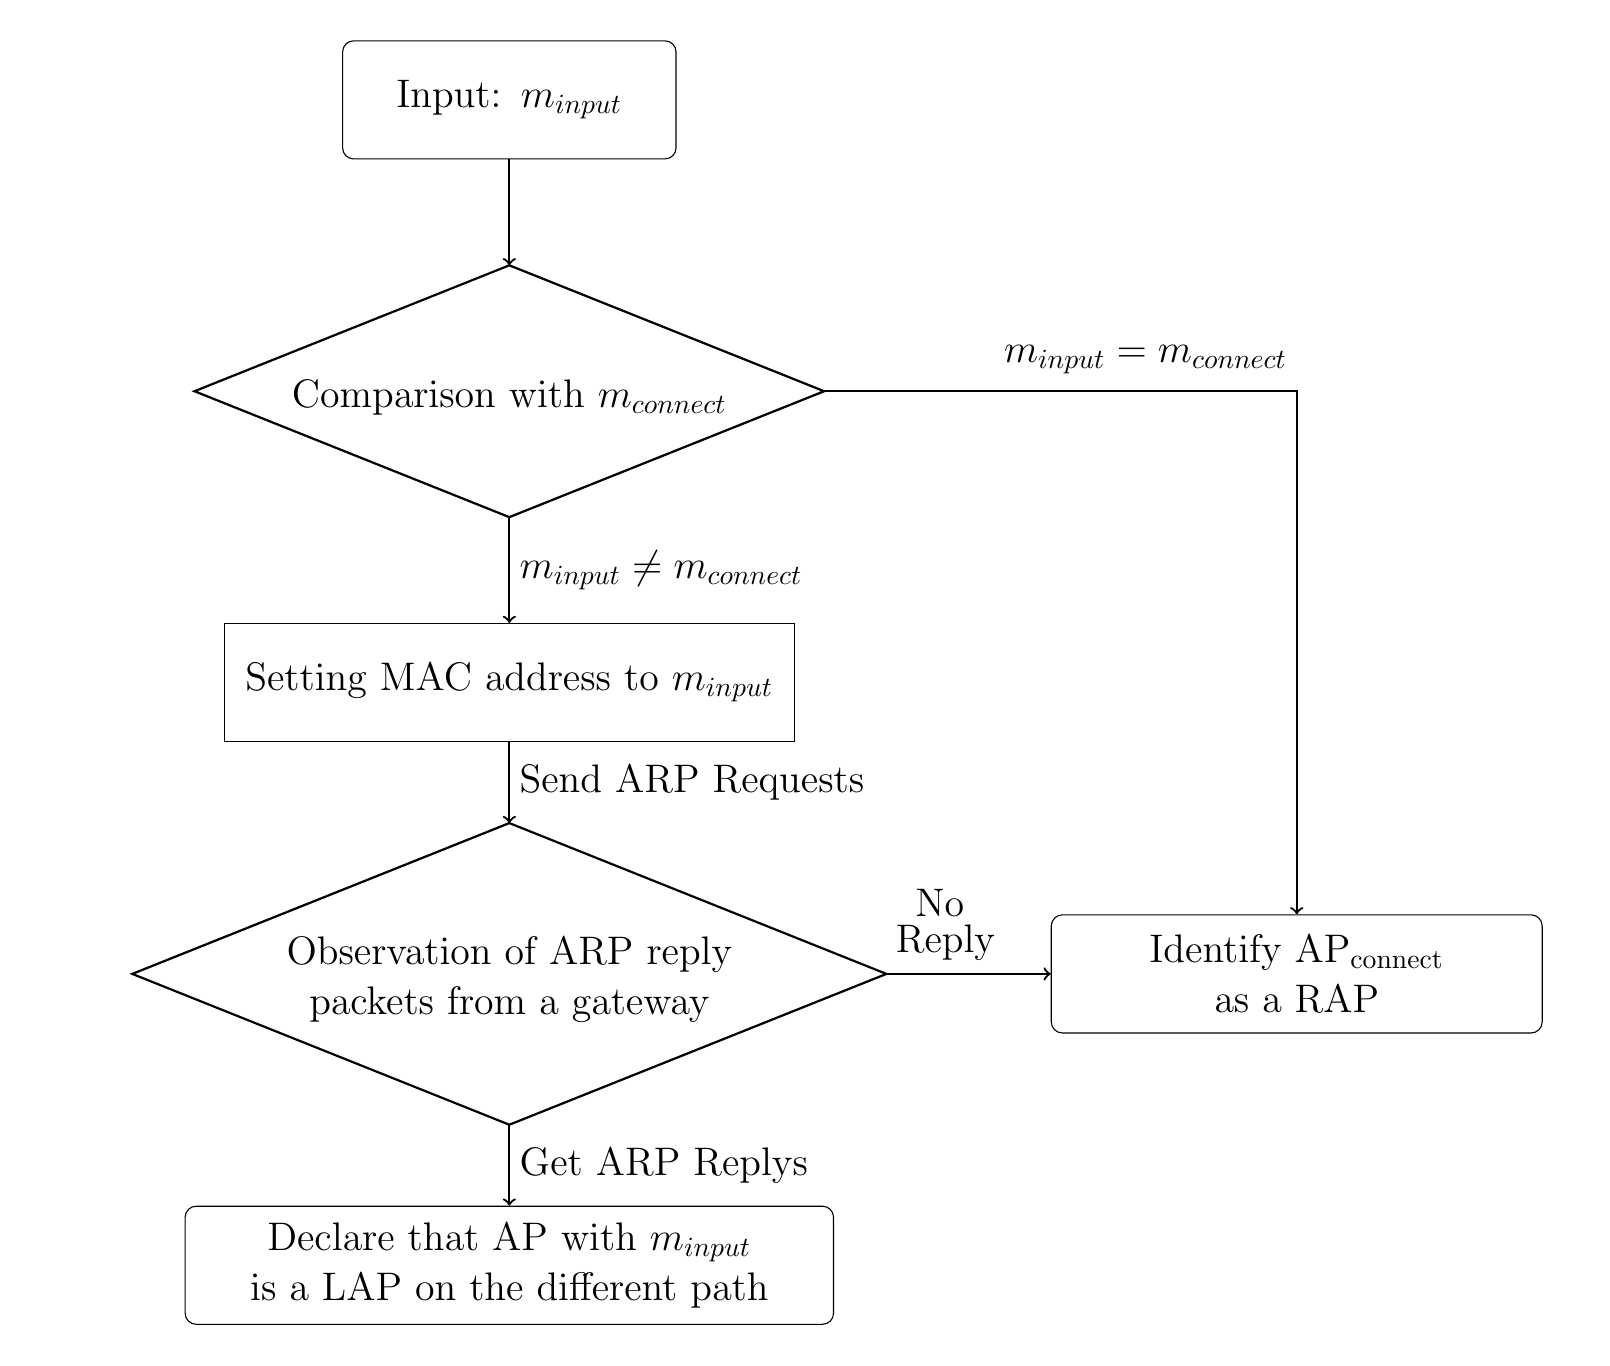
\begin{tikzpicture}[scale=1]
	\tikzset{block/.style={rectangle, draw, text width=7cm, font=\Large, text centered, minimum height=1.5cm}};
	\tikzset{empty/.style={rectangle}};
	\tikzset{init/.style={rectangle, draw, text width=4cm, rounded corners, font=\Large, text centered, minimum height=1.5cm}};
    \tikzset{end/.style={rectangle, draw, text width=8cm, rounded corners, font=\Large, text centered, minimum height=1.5cm}};
    \tikzset{end2/.style={rectangle, draw, text width=6cm, rounded corners, font=\Large, text centered, minimum height=1.5cm}};

    \tikzset{base/.style = {draw, thick, 
	text width=6.0cm, 
	text height=0.5cm, align=center, 
	inner sep=1mm, outer sep=0mm, 
	join=by arrow}};
	\tikzset{base2/.style = {draw, thick, 
	text width=4.5cm, 
	text height=0.5cm, align=center, 
	inner sep=1mm, outer sep=0mm, 
	join=by arrow}};
	\tikzset{decision/.style = {diamond, base,aspect=2.5, inner xsep=0mm, font=\Large}};
	\tikzset{decision2/.style = {diamond, base2,aspect=1.5, inner xsep=0mm, font=\Large}};
	\tikzset{declare/.style={rectangle, draw, text width=2.5cm,font=\Large, text centered, minimum height=1.0cm}};
	% Place nodes
	\node [empty](em) at (-3cm, 4cm){};
    \node [init] (init) at (0cm,3.2cm) {Input: $m_{input}$};
    \node [decision] (compare) at (0cm,-0.5cm) {Comparison with $m_{connect}$};
    \draw [thick, ->] (init) -- (compare);
    \node [block] (set) at (0cm, -4.2cm) {Setting MAC address to $m_{input}$};
    \draw [thick, ->] (compare) -- node[right] {\Large $m_{input} \ne m_{connect}$}(set);
    \node [decision] (observe) at (0cm, -7.9cm) {Observation of ARP reply packets from a gateway};
    \draw [thick, ->] (set) -- node[right]{\Large $\rm Send\ ARP\ Requests$} (observe);
    \node [end] (lap) at (0cm, -11.6cm) {Declare that AP with $m_{input}$  is a LAP on the different path};
    \draw [thick, ->] (observe) -- node[right]{\Large $\rm Get\ ARP\ Replys$}(lap);

    \node [end2] (rap) at (10cm, -7.9cm) {Identify $\rm AP_{connect}$ as a RAP};
    \draw [thick, ->] (observe) -- (rap);
    \draw [thick, ->] (compare) -| (rap);
	% \coordinate (sc) at (1.8cm, -11.6cm) node at (sc) [left] {\Large$\rm logo\ existence$};
	\node [empty](em) at (-6cm, -12.4cm){};
	\node [empty](em) at (13.5cm, -12.4cm){};

    \coordinate (m) at (10cm, -0.1cm) node at (m) [left] {\Large $m_{input} = m_{connect}$};
    \coordinate (m) at (5.9cm, -7.0cm) node at (m) [left] {\Large $\rm No$};
	\coordinate (m) at (6.3cm, -7.5cm) node at (m) [left] {\Large$\rm Reply$};
	%Place draw
	%\draw [thick, ->] (domain) -- node[right]{\Large $\rm Not\ Existed\ Domain$}(preparation);
	%\draw [thick, ->] (domain) -| (leg);

\end{tikzpicture}

\end{document}
 
